\chapter*{Simulación Basada en Agentes} \label{cap1}
\addcontentsline{toc}{chapter}{Simulación Basada en Agentes}

\begin{flushright}
\begin{minipage}{7.85cm}
    {\em Creo que para final de siglo el uso de las palabras y la opinión
    general habrán cambiado tanto, que uno podrá hablar sobre máquinas pensantes
    sin que le contradigan.} \\ Alan M. Turing
\end{minipage}
\end{flushright}

\vspace*{5mm}

\section{Agentes Inteligentes}

% http://en.wikipedia.org/wiki/Intelligent_agent#A_variety_of_definitions

Una posible definición muy resumida de agente inteligente sería la siguiente:
{\em un agente inteligente es una entidad autónoma que observa y actúa sobre un
entorno, y dirige su actividad en pos de uno o más objetivos}. Por supuesto
esta definición no abarca muchos matices, pero nos da una idea general que nos
sirve como punto de partida. La variedad de agentes es muy amplia, así como
su complejidad, que puede ir desde un sencillo agente puramente reactivo a uno
complejo que imite a una persona, por ejemplo.

Las siguientes características son necesarias para que un proceso sea
considerado un agente de algún tipo\cite{Macal06}:

\begin{itemize}
 \item Un agente es indentificable; tiene límites definidos, por lo que es fácil
 determinar cuando algo es parte del agente, no lo es, o es un característica
 compartida.
 \item Un agente está situado en un entorno con el que interactúa, y en caso de
 tratarse de un sistema multiagente, y en el que convive con otros agentes con
 los que también se comunica.
 \item Un agente ha de ser autónomo, capaz de funcionar sin requerir la
 intervención del usuario.
\end{itemize}

Los agentes se pueden clasificar según sus características y habilidades, no
todos los agentes son igual de complejos ni todos pueden considerarse {\em
inteligentes}.

\begin{figure}[H]
 \centering
 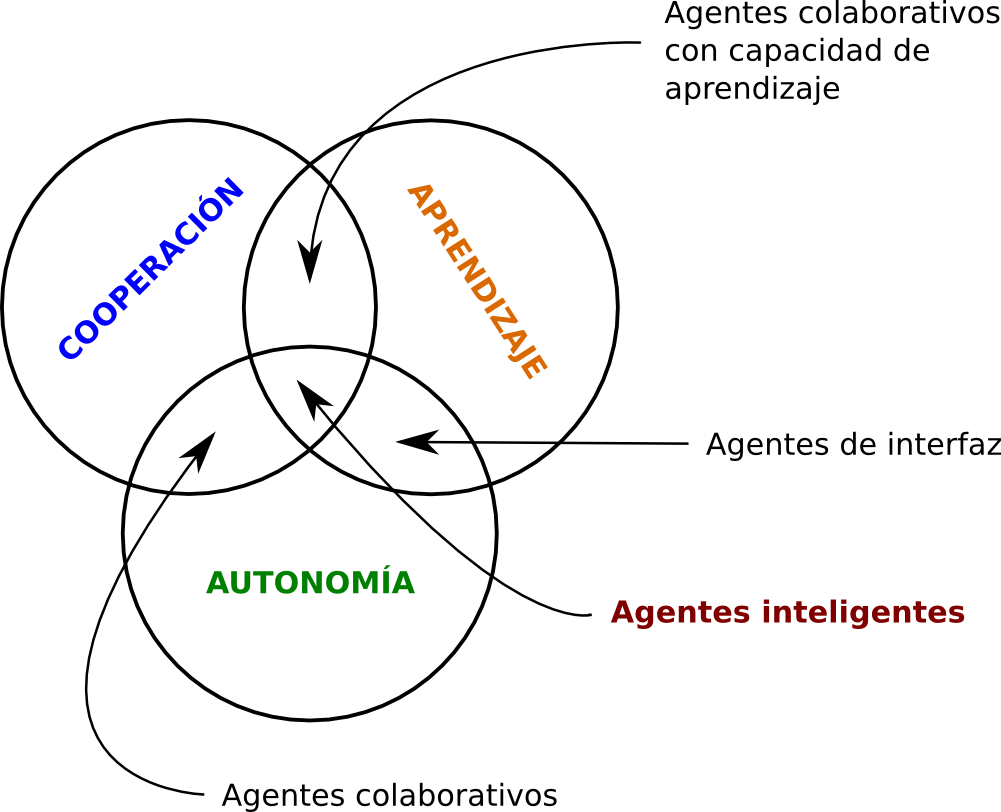
\includegraphics[width=120mm]{figuras/cap1/tipos_agentes.png}
 \caption{Tipos de agentes}
\end{figure}

Existen muchas definiciones de agentes inteligentes, todas ellas diferentes,
pero con puntos en común. Los puntos que se pueden extraer como fundamentales
para considerar a un proceso como {\bf agente inteligente} son:

\begin{description}
 \item[Autonomía]Deben ser capaces de funcionar sin la intervención del usuario.
 \item[Reactividad]Han de poder observar su entorno, y responder a los eventos
 o cambios que se produzcan.
 \item[Proactividad]Para conseguir sus objetivos han de tomar decisiones y
 realizar acciones según una estrategia.
 \item[Comunicación]Deben poder comunicarse entre sí, compartir información, e
 incluso, cooperar para la consecución de sus objetivos.
\end{description}

Aunque existen agentes puramente reactivos, es difícil aplicarles la etiqueta
de {\em inteligentes}. Un grado de proactividad es imprescindible, aunque se
hace necesario encontrar un equilibrio entre la reactividad y la búsqueda
activa de objetivos.

\subsection{Qué no es un Agente}

% http://en.wikipedia.org/wiki/Software_agent#What_an_agent_is_not

A veces resulta más claro y práctico comparar lo que se quiere definir con
elementos relacionados y resaltar las diferencias, que dar una definición. A
continuación sigue una comparación entre un agente inteligente y otros tipos de
software relacionados.

\subsubsection{Agentes frente a Programas}

Las principales características que distinguen a un agente de un programa
arbitrario son cuatro: {\em reactividad al entorno, autonomía, proactividad y
persistencia}\cite{Franklin96}.

\subsubsection{Agentes frente a Objetos}

Las diferencias que intuitivamente se pueden encontrar son las
siguientes\cite{Wooldridge95}:

\begin{itemize}
 \item Los agentes son más autónomos que los objetos.
 \item Los agentes tienen un comportamiento más flexible, reactivo, proactivo
 y social.
 \item Los agentes tienen como mínimo un hilo de control, pero pueden tener más.
\end{itemize}

\subsubsection{Agentes frente a Sistemas Expertos}

Las diferencias son las siguientes\cite{Wooldridge95}:

\begin{itemize}
 \item Los sistemas expertos no están emparejados a su entorno.
 \item Los sistemas expertos no están diseñados para tener un comportamiento
 reactivo ni proactivo.
 \item Los sistemas expertos no tienen capacidades sociales.
\end{itemize}

\subsection{Tipos de Agentes}

Existen varios tipos de agentes según sus características y capacidades. Lo que
sigue es sólo una de las posibles clasificaciones.

\subsubsection{Reactivos}

Los agentes puramente reactivos actúan únicamente en base a su percepción. La
funcionalidad del agente está basada en {\em la regla de condición-acción}: si
tal condición entonces tal acción. Este tipo de agentes es particularmente
interesante cuando el entorno es observable en su totalidad.

También es posible que un agente reactivo contenga información de su estado en
cada momento, lo que les permite obviar {\em condiciones} que ya hayan activado
{\em acciones} en momentos anteriores.

\subsubsection{Reactivos basados en Modelo}

Este tipo de agentes es capaz de desenvolverse en entornos que son sólo
parcialmente observables. Almacenan su estado en cada momento manteniendo algún
tipo de estructura que describa el entorno que no se puede percibir.
Obviamente, esta cualidad requiere información sobre como se comporta y
funciona el entorno. Es esta información adicional la que completa las
percepciones del agente.

Un agente reactivo basado en modelo realiza un seguimiento del estado del
entorno en cada momento, usando su modelo interno. Con ambas informaciones (su
modelo interno y sus percepciones) toma las decisiones de la misma manera que un
agente puramente reactivo.

\subsubsection{Basados en Objetivos}

Los agentes basados en objetivos son agentes basados en modelo que además
almacenan información relativa a situación que son deseables. Gracias a esto el
agente es capaz de escoger de entre múltiples posibilidades aquellas que
cumplen un objetivo.

\subsubsection{Basados en Utilidad}

Loa agentes basados en objetivos sólo diferencian entre estados objetivo y no
objetivo. Es posible definir una medida de cuan deseable es un estado en
particular. Esta medida se obtiene a través del uso de una función de
evaluación de la {\em utilidad} de un estado concreto.

Gracias a esta función el agente es capaz de escoger aquellos estados que
ayudan o favorecen la consecución de los objetivos, en el caso de que ningún
estado posible cumpla un objetivo directamente.

\subsubsection{Con capacidad de Aprendizaje}

El aprendizaje presenta ventajas tales como que permite a los agentes operar en
entornos inicialmente desconocidos, y convertirse en agentes más competentes
de lo que su conocimiento inicial por sí mismo permitiría. Esta capacidad de
aprendizaje requiere que el agente tenga memoria, y permite la mejora de la
eficacia de éste a lo largo del tiempo.

\section{Sistemas MultiAgente (SMA)}

% http://en.wikipedia.org/wiki/Multi-agent_system

Un sistema multiagente (SMA) es un sistema compuesto de múltiples agentes
inteligentes que interactúan entre sí. Estos sistemas se utilizan para resolver
aquellos problemas que son complicados, o directamente imposibles, para un único
agente o un sistema monolítico.

Para que un sistema pueda ser considerado un SMA es necesario que se cumplan
las siguientes condiciones:

\begin{itemize}
 \item Los agentes han de ser al menos parcialmente autónomos.
 \item Ningún agente debe tener una visión completa y global del sistema, o
 bien el sistema es tan complejo que ningún agente podría hacer un uso práctico
 de un conocimiento completo.
 \item No puede haber un agente designado para controlar el sistema al
 completo, pues se convertiría en un sistema monolítico.
\end{itemize}

En un SMA puede manifestarse un comportamiento emergente complejo y sofisticado,
incluso cuando las estrategias individuales de sus agentes sean simples y
sencillas.

Los agentes de un SMA pueden comunicarse entre sí y compartir conocimiento, con
las limitaciones que imponga el protocolo de comunicación del sistema.

\subsection{Cuándo utilizar un SMA}

Los sistemas multiagente son especialmente útiles cuando se da alguna, o varias,
de las siguientes situaciones\cite{Bonabeau02}:

\begin{itemize}
 \item Cuando las interacciones entre los agentes son complejas, no lineales,
 discontinuas, o discretas.
 \item Cuando la posición es crucial y no es fija.
 \item Cuando la población es heterogénea, cuando cada individuo es
 (potencialmente) diferente.
 \item Cuando la topología de la interacción es heterogénea y compleja.
 \item Cuando los agentes requieren comportamientos complejos, incluyendo
 aprendizaje y adaptación.
\end{itemize}

\subsection{Estrategia de Trabajo}

Existen múltiples formas de plantear un sistema multiagente, pero una de la más
habituales es la técnica de {\em divide y vencerás}. Básicamente se trata de
subdividir el problema en problemas más pequeños resolubles por agentes
particulares, o bien por un subconjunto de agentes que cooperen entre sí.

La solución global surgiría de la combinación del trabajo de cada agente, esta
supersolución puede surgir de manera automática como un comportamiento
emergente, o puede ser necesario que otro agente explícitamente se encargue de
elaborarla.

El principal obstáculo a la hora de aplicar esta técnica es que los problemas
normalmente no tienen una solución general. Muchas veces se ha necesario
resolver cada caso por separado, lo que puede conducir a comportamientos
erróneos o a la aparición de comportamientos emergentes no deseados.

\subsection{Protocolos de Comunicación}

Es la capacidad de comunicación entre los agentes que componen un SMA lo que
permite que el sistema funcione y resuelva problemas. Sin comunicación no hay
SMA.

Existen varios métodos de comunicación entre agentes, pero el más habitual es
el paso de mensajes entre ellos. Para poder llevar esto a cabo es necesario
definir protocolos de comunicación, y dos de los más utilizados son el {\em
Knowledge Query Manipulation Language
(KQML)}\footnote{\url{http://www.cs.umbc.edu/research/kqml/}} y el {\em Agent
Communication Language
(ACL)}\footnote{\url{http://www.fipa.org/repository/aclspecs.html}}.

Es muy importante que estos protocolos se estandaricen para poder establecer
interacciones entre diferentes plataformas de agentes.

%%% Local Variables:
%%% mode: latex
%%% TeX-master: "../dissim"
%%% End: